\documentclass[../thesis.tex]{subfiles}
% Separate preamble for this subfile. This preamble is loaded last, so one can override various functions before \begin{document}

% Better comment extension for Vscode colors these comments differently
% Normal comment color
% * Important information
% ! ALERT
% ? Question
% TODO stuff to do
% // This is strikethrough


\begin{document}

Informally, to tile refers to the process of covering some surface with objects. These objects are called tiles and come in a variety of shapes and sizes. When we are tiling, we essentially place copies of the tile next to each other in a systematic way, intending to leave no gaps and no overlaps between the tiles \cite{kolountzakisTilingsTranslation2010}. The resulting tiling can be as simple as the one shown in \cref{fig:tiling_one} where we have used a single tile, the unit square, to tile the plane, or as complex as \cref{fig:tiling_two} where we have used four different tiles to tile the plane. The first is an example of what is known as a \emph{monohedral tiling} in which all tiles are congruent \cite[p. 20]{grunbaumTilingsPatterns1987}, and the latter is an example of a Penrose tiling which are well known for being non-periodic \cite{penrosePentaplexityClassNonPeriodic1979}. %* 1979 page 535 har også penrose tilings




\begin{figure}[h!]%h!
    \centering
    \begin{subfigure}{.47\textwidth}
        \centering
        %\includegraphics[width=0.9\linewidth]{spec_no_shift.jpg}
        %* Figure 1
        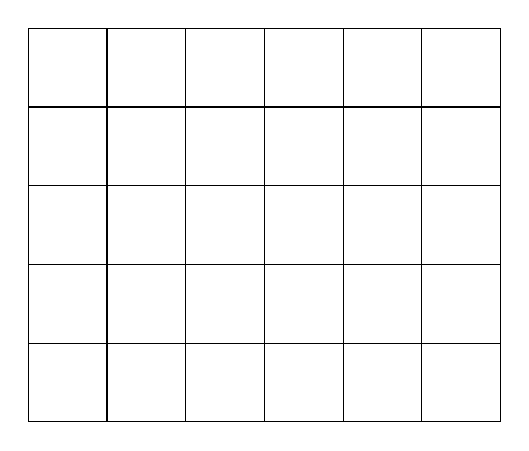
\begin{tikzpicture}[scale=1]
            % Define the tile
            \def\tile{
              % Draw the unit square
              \draw (0,0) rectangle (1,1);
            }
          
            % Draw the tiling pattern
            \foreach \x in {0,1,2,3,4,5}{
              \foreach \y in {0,1,2,3,4}{
                \pgfmathsetmacro{\shiftX}{\x} % Set horizontal shift
                \pgfmathsetmacro{\shiftY}{\y} % Set vertical shift
                \begin{scope}[shift={(\shiftX,\shiftY)}]
                  \tile % Draw the tile
                \end{scope}
              }
            }
        \end{tikzpicture}
        %* —————————————————
        \caption{Lattice spectra}
        \label{fig:tiling_one}
    \end{subfigure}\quad
    \begin{subfigure}{.47\textwidth}
        \centering
        \includegraphics[width=0.9\linewidth]{Penrose_Tiling_.png}
        \caption{P1 Penrose Tiling}
        \label{fig:tiling_two}
    \end{subfigure}
    \caption{Penrose original aperiodic tiling \cite{penrosePentaplexityClassNonPeriodic1979}, from \cite{inductiveloadP1TilingUsing}, forklare fargelegginen, \SigridComment{By Inductiveload - Own work, Public Domain, https://commons.wikimedia.org/w/index.php?curid=5839133}}
    \label{fig:tilingsss}
\end{figure}


Another interesting pair of monohedral tilings is given in \cref{fig:tiling_three,fig:tiling_four}. These are both examples of an Escher tiling in which a lizard and horseman tile the plane. Note that in comparison to the square tilings in \cref{fig:tiling_one}, there is important to highlight two fundamental differences between the square and Escher tilings. The first is that one needs to rotate the lizard to cover the entire surface, and the second is that one needs to reflect the horseman to cover the entire surface. It is these three motions and combinations of them that we use when tiling in general \cite[p. 26]{kolountzakisTilingsTranslation2010,grunbaumTilingsPatterns1987}. 


\begin{figure}[t]%h!
    \centering
    \includegraphics[width=0.4\linewidth]{lizard-1.jpg}
    \caption{Lizard from \cite{m.c.escherLizard1942}}
    \label{fig:tiling_three}
\end{figure}


\mycomment{  %! Block comment
\begin{figure}[t]%h!
    \centering
    \begin{subfigure}{.47\textwidth}
        \centering
        \includegraphics[width=0.9\linewidth]{lizard-1.jpg}
        \caption{Lizard}
        %\label{fig:tiling_three}
    \end{subfigure}\quad
    \begin{subfigure}{.47\textwidth}
        \centering
        \includegraphics[width=0.9\linewidth]{flying-fish.jpg}
        \caption{Flying fish}
        \label{fig:tiling_four}
    \end{subfigure}
    \caption{from \cite{m.c.escherLizard1942}}
    \label{fig:tilingsss_two}
\end{figure}
}

However interesting the Penrose and Escher tilings appear, we will only focus on tilings of $\R^d$ by translation and using only the unit cube as our tile. Considering only cube-tilings might seem simple initially, but we will see that as we increase the dimension, we get increased flexibility and more complex tilings. It turns out that in higher dimensions, highly exotic and counterintuitive cube tilings exist. The fact that this kind of tiling exists in the first place is surprising in light of Keller's theorem \cite{iosevichSpectralTilingProperties1998}.  % This is Perhaps surprising in light of Keller's theorem. 

%\begin{theorem}  %* (My original) Keller theorem from the paper of Iosovich and Pedersen
%    Given a discrete subset $T\subset \R^d$. If $T$ is a tiling set for $\Omega$, then given any pair $\lambda, \lambda' \in T$ such that $\lambda\neq\lambda'$, there exists a $j\in \braq{1,\dots,d}$ so that $\bral{t_j -t_j' } \in \N$
%\end{theorem}
%\begin{theorem}  %* Keller theorem from the paper of Lagarias and Reeds
%    If $\Lambda + \bras{0,1}^n$ is a tiling of $\R^n$, then each $\lambda,\lambda'\in \Lambda$ has
%    \begin{equation*}
%        \lambda_i - \lambda_i' \in \intnozero \quad \text{ for some } i, \quad 1\leq i \leq n.
%    \end{equation*}
%\end{theorem}
\begin{theorem}[Keller's Theorem]\label{thrm:keller_tiling}
    %Let $\Lambda \subset \R^d$ be a discrete subset.  %* No need to specify, as we will define the tiling set later
    If $\Lambda$ is a tiling set for the unit cube $I^d$, then for any two $\lambda, \lambda' \in \Lambda$ with $\lambda\neq\lambda'$, there exist a $j\in \braq{1,\dots,d}$ so that $\lambda_j-\lambda_j' \in \intnozero$.
\end{theorem}

We will formally define what we mean by a \emph{tiling set} from \cref{thrm:keller_tiling} later (\cref{def:tiling}), but for now, we continue this informal discussion on exotic tilings. Now, although Keller proved the theorem in his original paper \cite{kellerUberLuckenloseErfullung1930}, Iosevich and Pedersen provide an English proof in their paper \cite{iosevichSpectralTilingProperties1998}. Furthermore, in the same paper by Keller, he also conjectured the following. 

\begin{conjecture}[Keller's conjecture]\label{conj:keller_tiling}
    All tilings of $\R^d$ by translations of the unit cube contain \textsc{two} cubes that share an entire $(d-1)$-dimensional face.
\end{conjecture}  %* For å kaste lys på at de kan være eksotiske så er det det at de er usant over 7 som er det relevante her. 

\input{figures/figure-tex/tiling_three.tex}

If the dimension is two, the squares share an edge; if the dimension is three, they share a square. \cref{fig:tilings_five_six} illustrates this. Furthermore, when $d\geq 3$, it is not necessarily true that \emph{all} cubes shared a whole $(n-1)$-dimensional face with one of its neighbors \cite{perronUeberLueckenloseAusfuellung1940}. It is important to emphasize that the conjecture does not support the existence of exotic tilings. Instead, it indicates the opposite — rigidity in the tiling of the space. %/ $\R^d$.
However, after being first proven true for $d\leq 6$ by Perron in 1940 \cite{perronModulartigeLueckenloseAusfuellung1940,perronModulartigeLueckenloseAusfuellung1940a}, it has since then gradually been proved false for all $d\geq10$ \cite{lagariasKellerCubetilingConjecture1992} and later all $d\geq8$ \cite{mackeyCubeTilingDimension2002}. The last remaining dimension was finally solved in 2020, where it was proven to be true \cite{brakensiekResolutionKellerConjecture2020}, leading us to a solution in all dimensions for Keller's \namecref{conj:keller_tiling}.%, \cref{conj:keller_tiling}. 

\begin{theorem}
    In all tilings of $\R^d$ by translations of the unit cube, Keller's \namecref{conj:keller_tiling}, \cref{conj:keller_tiling}, is true for all dimensions $d\leq 7$ and false for all $d>7$.
\end{theorem}
It is precisely the higher dimensional tilings that counterexample Keller's conjecture that we intuitively \SigridChange{define/understand} to be the exotic and counterintuitive tilings.

\begin{remark}
    Keller also wrote a paper claiming to solve his conjecture for $d\leq 6$ \cite{Keller1937}. However, Perron later described Keller's solution for $d=5$ and $d=6$ as \emph{"quite incomprehensible to me"} and \emph{"very sketchy"} in the literal sense of the word \cite{perronUeberLueckenloseAusfuellung1940} \footnote[1]{Perron's origninal description of Keller's solution to his conjecture: \emph{— Enthält einen sehr skizzenhaften mir ziemlich unverständlichen Beweis für die Richtigkeit der Kellerchen Vermutung im Falle n=5 unt n=6.}}. Furthermore, what is interesting is the fact that Keller himself later doubted whether his conjecture was actually true.
\end{remark}
%* ———————————————————————————— Tilings ——————————————————
% In defining tilings formally, we use indicator functions \cite{kolountzakisTilingsTranslation2010}. 
% In defining tilings more formally/rigorously/using our geometric intuition/$\dots$,
% In defining a tiling more formally, one intuitive way is to define it as a non-overlapping covering of the space.
% One possible approach to providing a more formal definition of a tiling is to define it as a non-overlapping covering of the space.
\SigridComment{More grand statement of tilings?}\\
- Now, we endeavor to establish a more rigorous definition of tiling. One possible approach is to define it as a non-overlapping covering of the space.\\
- Now, in defining a tiling more formally, one possible approach is to define it as a non-overlapping covering of the space.\\ 

By this, we mean that a subset $\Omega \subset \R^d$ of non-zero measure is a tile, and a set $\Lambda \subset \R^d$ is a tiling set if they satisfy both of the following conditions. First, $\Omega+\lambda$ for $\lambda \in \Lambda$ must cover $\R^d$ up to measure zero. Secondly, all intersections $(\Omega+\lambda) \cap (\Omega+\lambda')$ of distinct elements $\lambda,\lambda' \in \Lambda$ must have measure zero. Note that $\Omega+\lambda$ denotes the translate of $\Omega$ by the vector $\lambda$. However, instead of the more intuitive geometric definition, we use the following as our working \namecref{def:tiling} in terms of indicator functions \cite{kolountzakisTilingsTranslation2010,kolountzakisStructureTilingsLine1996}.  % - However, instead of the more intuitive geometric definition, we use the following as our working definition in terms of indicator functions \cite{kolountzakisTilingsTranslation2010,kolountzakisStructureTilingsLine1996}.
% - More formally/Nevertheless, tilings can also be expressed using indicator functions as follows \cite{kolountzakisTilingsTranslation2010}. \SigridChange{/} We will, however, define tilings in terms of indicator functions as follows \cite{kolountzakisTilingsTranslation2010} \cite{kolountzakisStructureTilingsLine1996}.
% - Rather than defining tiling in terms of a non-overlapping covering of the space, we will instead define tiling by the indicator function, using little of our geometric intuition \cite{kolountzakisTilingsTranslation2010} \cite{kolountzakisStudyTranslationalTiling2003}. 
\begin{definition}[Tiling set]\label{def:tiling}
    Let $\Omega \subset \R^d$ be a subset with non-zero measure, and consider a discrete set $\Lambda \subset \R^d$. If
    \begin{equation}\label{eq:tiling_set}
        \sum_{\lambda \in \Lambda} \indicator{\Omega}{x-\lambda} = 1, \quad a.e. \text{\space\space} x \in \R^d.
    \end{equation}
    then $\Omega$ is called a \emph{tile}, and $\Lambda$ is called a \emph{tiling set} for $\Omega$. We say that $(\Omega, \Lambda)$ is a \emph{tiling pair}.
\end{definition}
\begin{remark}
    We can also say that $\Omega$ \emph{tiles $\R^d$ by translation}, or that $\Omega$ is a \emph{tiling} of $\R^d$. 
\end{remark}
\begin{remark}
    Additionally, one can define tilings more generally. By this, we mean that in place of the indicator function, we can have a non-negative, integrable function $f$. Other than allowing for any other constant value than $1$, the definition is the same. The reader is referred to \cite{kolountzakisTilingsTranslation2010,kolountzakisStructureTilingsLine1996} for more details on this topic.
\end{remark}
% Direct in text:
% In other words, we can also say that $\Omega$ \emph{tiles $\R^d$ by translation}, or that $\Omega$ is a \emph{tiling} of $\R^d$. Additionally, one can define tilings more generally. By this, we mean that in place of the indicator function, we can have a non-negative, integrable function $f$. Other than allowing for any other constant value than $1$, the definition is the same. Note that we still require the same constant value almost everywhere. The reader is referred to \cite{kolountzakisTilingsTranslation2010} for more details on this topic.
%* ———————————————————————————— One dimension  ——————————————————
%* Viktig, må inn en bit her om 
%* som en konsekvens av Kellers theorem så får vi nå akkurat den samme formen på disse tilings settene 
%* de må ligge inneholt i akkurat de samme typene mengder, og de kan ikke være ekte mindre for da får vi ikke oppfylt tiling kravet mitt.
If we now restrict our attention to the unit cube in $d$-dimensions, Keller's theorem immediately gives the following for $d=1$. Here, the unit cube is simply the unit interval $I = \bras{0,1}$. %In dimension one, the unit cube is simply the unit interval $I = \bras{0,1}$. 

\begin{lemma}\label{lem:tiling_unit_1d}
    %The set $\Lambda = \Z +\alpha$ for some value $\alpha\in \R$ constitutes a tiling set for $I$.
    %The only subsets $\Lambda \in \R$ such that $\Lambda$ is a tiling set for $I$ are $\Lambda = \Z +\alpha$ for some value $\alpha\in \R$.
    The only subsets $\Lambda \in \R$ such that $\Lambda$ is a tiling set for $I$ are the translates $\Lambda = \Z +\alpha$ for a fixed value $\alpha\in \R$. 
\end{lemma}

\begin{proof}  % This follows directly from \cref{thrm:keller_tiling}. Take $\lambda, \lambda' \in \Lambda$. 
    %  Må konkret gå tilbake til definisjonen du har valgt. For den kan vi bruke eksplisitt til å si:
    %Det Keller's theorem forteller meg, er at jeg må ha noe som er en undermengde av $\Lambda = \Z + \alpha$, og i og med at jeg må ha 1 almost everywhere, så gjør det at hvis jeg tar bort et punkt fra $\Lambda$ slik at vi har $\Lambda \subset \Z + \alpha$, så vil jeg få et intervall hvor jeg har 0.
    %  La oss nå si at et punkt er utelatt. Det betyr at $\sum \indicator{\Omega}{t} = 0$ og vi kan si nøyaktig hvor det er null, for det er på det punktet vi har utelatt. Dvs, $x\in I+\lambda'$, hvor $\lambda'$ er punktet vi utelot fra flisleggingsmengden. Videre, så er målet av $I+\lambda'$ positivt, det er ikke neglisjerbart. Dvs, der du ikke har verdien 1, de områdene, de er ikke neglisjerbare. Og videre vet vi at vi har $x\in I+\lambda'$, dvs et helt slikt interval, hvor $\sum \indicator{\Omega}{t} = 0$, og dette området har positivt mål. 
    Let $\Lambda \subset \R^d$. Using Keller's theorem, \cref{thrm:keller_tiling}, we instantly get that there must be an integer distance between two distinct points $\lambda,\lambda' \in \Lambda$ if $\Lambda$ is to be a tiling set for $I$. Hence, we know that $\Lambda \subseteq \Z +\alpha$ for a fixed $\alpha\in \R$. Now, given an arbitrary point $\lambda' \in \Z +\alpha$, assume that $\lambda'\notin \Lambda$ so that we have a case where $\Lambda \subset \Z+\alpha$. However, by using \cref{def:tiling}, observe now that we have an entire interval, specifically $I+\lambda'$, where $\indicator{I}{x - \lambda'} = 0$. As $\mes{I+\lambda'} = 1 $, this is non-negligible, and we do not achieve
    \begin{equation*}
        \sum_{\lambda \in \Lambda\setminus \braq{\lambda'}} \indicator{I}{x-\lambda} = 1, \quad a.e. \text{\space\space} x \in \R^d.
    \end{equation*}
    %* As $\mes{I+\lambda'} = 1 $, this is non-negligible, and we do not achieve $\indicator{I}{x-\lambda} = 1$ almost everywhere for $x\in\R^d$ with the set $\Lambda\setminus \braq{\lambda'}$. % In short: That is, we have a non-negligible region with a value not equal to one.
    Hence $\lambda' \in \Lambda$, which shows that $\Lambda = \Z+\alpha$. This concludes the proof that there are no other tiling sets for $I$ in dimension $d=1$. %and that $\Lambda$ is a tiling set for $I$ . %for a tiling set $\Lambda$ of
\end{proof}

Increasing the dimension by one, we get more flexibility. We do not necessarily need to have a lattice tiling as the one in \cref{fig:tiling_one}. We can have tilings where we translate single or multiple \emph{columns} of the unit cube, shown in \cref{fig:single_shift_vertical_tiling,fig:multiple_shift_vertical_tiling}; or single or multiple \emph{rows} of the unit cube, shown in \cref{fig:single_shift_horizontal_tiling,fig:multiple_shift_horizontal_tiling}. We will see later in \cref{chap:equivalence} that \cref{fig:tiling_figures} to some extent fully captures the flexibility of two dimensions. We remark that all \cref{fig:single_shift_vertical_tiling,fig:multiple_shift_vertical_tiling,fig:single_shift_horizontal_tiling,fig:multiple_shift_horizontal_tiling} clearly illustrates that all tilings for $d=2$ also satisfy Keller's theorem. 




\begin{figure}[t]%h!
    \centering
    \begin{subfigure}{.47\textwidth}
        \centering
        %\includegraphics[width=0.9\linewidth]{spec_no_shift.jpg}
        %* Figure 1
        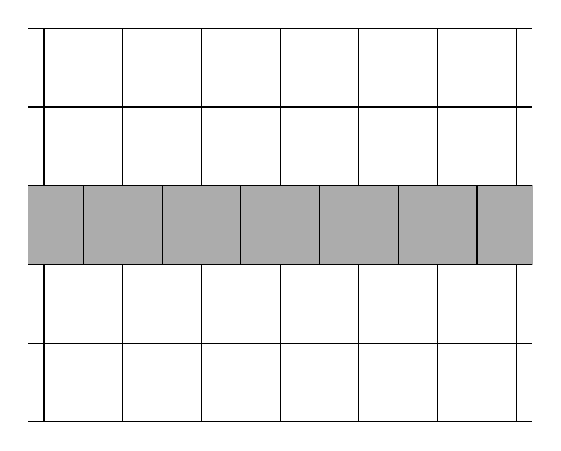
\begin{tikzpicture}[scale=1]
            % Define the tile
            \def\tile{
            \draw[fill=white] (0,0) rectangle (1,1);
            }
            \def\tiletwo{
            \draw[fill=gray!65] (0,0) rectangle (1,1);
            }
            
            % Draw the tiling pattern
            % Everything else
            \foreach \y in {0,1,3,4}{
                \foreach \x in {0,1,2,3,4,5}{
                    \pgfmathsetmacro{\shiftX}{\x} % Set horizontal shift
                    \pgfmathsetmacro{\shiftY}{\y}
                    \begin{scope}[shift={(\shiftX,\shiftY)}]
                        \tile
                    \end{scope}
                }
            }
            % Shifted line
            \foreach \x in {0}{
            \draw[gray!65, fill=gray!65] (\x-0.2,2) rectangle (\x+0.5,3);
            }
            \foreach \x in {6}{
            \draw[gray!65, fill=gray!65] (\x+0.2,2) rectangle (\x-0.5,3);
            }
            % Middle line, must be after the above code in order to get black lines at correct spots
            \foreach \y in {2}{
                \foreach \x in {0,1,2,3,4}{
                    \pgfmathsetmacro{\shiftX}{\x+0.5} % Set horizontal shift
                    \pgfmathsetmacro{\shiftY}{\y}
                    \begin{scope}[shift={(\shiftX,\shiftY)}]
                        \tiletwo
                    \end{scope}
                }
            }
            % small black lines at the top and bottom
            \foreach \y in {0,1,2,3,4,5}{
                \draw (0-0.2,\y) -- (6+0.2,\y);
            }
        \end{tikzpicture}
        %* —————————————————
        \caption{Single row shift}
        \label{fig:single_shift_horizontal_tiling}
    \end{subfigure}\quad
    \begin{subfigure}{.47\textwidth}
        \centering
        %\includegraphics[width=0.9\linewidth]{spec_single_shift.jpg}
        %* Figure 2
        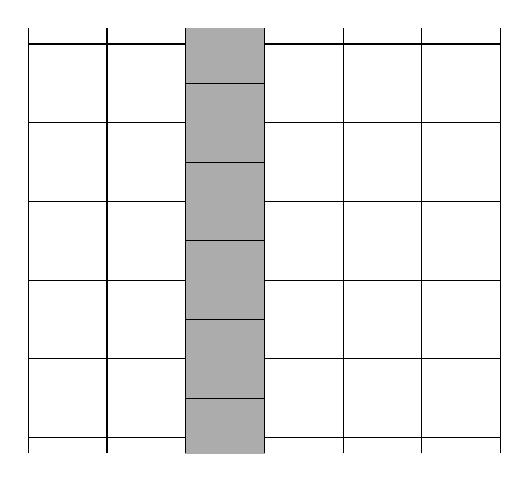
\begin{tikzpicture}[scale=1]
            % Define the tile
            \def\tile{
            \draw[fill=white] (0,0) rectangle (1,1);
            }
            \def\tiletwo{
            \draw[fill=gray!65] (0,0) rectangle (1,1);
            }
            
            % Draw the tiling pattern
            % Everything else
            \foreach \x in {0,1,3,4,5}{
                \foreach \y in {0,1,2,3,4}{
                    \pgfmathsetmacro{\shiftX}{\x} % Set horizontal shift
                    \pgfmathsetmacro{\shiftY}{\y}
                    \begin{scope}[shift={(\shiftX,\shiftY)}]
                        \tile
                    \end{scope}
                }
            }
            % Shifted line
            \foreach \y in {0}{
            \draw[gray!65, fill=gray!65] (2,\y-0.2) rectangle (3,\y+0.5);
            }
            \foreach \y in {5}{
            \draw[gray!65, fill=gray!65] (2,\y+0.2) rectangle (3,\y-0.5);
            }
            % Middle line, must be after the above code in order to get black lines at correct spots
            \foreach \x in {2}{
                \foreach \y in {0,1,2,3}{
                    \pgfmathsetmacro{\shiftX}{\x} % Set horizontal shift
                    \pgfmathsetmacro{\shiftY}{\y+0.5}
                    \begin{scope}[shift={(\shiftX,\shiftY)}]
                        \tiletwo
                    \end{scope}
                }
            }
            % small black lines at the top and bottom
            \foreach \x in {0,1,2,3,4,5,6}{
                \draw (\x,0-0.2) -- (\x,5+0.2);
            }
        \end{tikzpicture}
        %* —————————————————
        \caption{Single column shift}
        \label{fig:single_shift_vertical_tiling}
    \end{subfigure}\\
    \begin{subfigure}{.47\textwidth}
        \centering
        %\includegraphics[width=0.9\linewidth]{multiple_shift_left_zero.jpg}
        %* Figure 3
        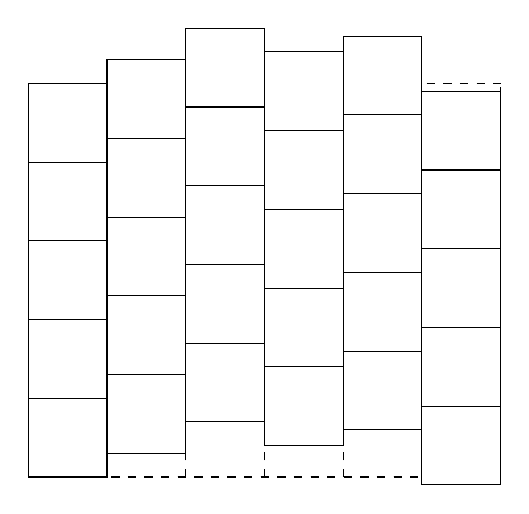
\begin{tikzpicture}[scale=1]
            % Define the tile
            \def\tile{
            % Draw the unit square
            \draw[fill=white] (0,0) rectangle (1,1);
            }

            % Shift list
            \def\BetaMinOne{0}
            \def\BetaZero{0.3}
            \def\BetaOne{0.7}
            \def\BetaTwo{0.4}
            \def\BetaThree{0.6}
            \def\BetaFour{-0.1}
            
            

% Axis lines
%\draw[->] (-1.5,0) -- (4.5,0) node[right] {$X$};
%\draw[->] (0,-1.5) -- (0,3.5) node[above] {$Y$};
\draw[dashed] (0,0) -- (6,0);
\draw[dashed] (0,0) -- (0,5);

% Dashed lines at each integer in the x direction
\foreach \x in {0,...,6}
    \draw[dashed] (\x,0) -- (\x,5);

% Dashed lines at each integer in the y direction
\foreach \y in {0,...,5}
    \draw[dashed] (0,\y) -- (6,\y);


            % Draw the tiling pattern
            \foreach \x in {0,1,2,3,4,5}{
            \foreach \y in {0,1,2,3,4}{
                \ifnum\x=0 % Set vertical shift for the third column only
                    \pgfmathsetmacro{\shiftX}{\x} % No vertical shift for other columns
                    \pgfmathsetmacro{\shiftY}{\y + \BetaMinOne} % Shift one unit upward
                \fi
                \ifnum\x=1
                    \pgfmathsetmacro{\shiftX}{\x}
                    \pgfmathsetmacro{\shiftY}{\y + \BetaZero}
                \fi
                \ifnum\x=2
                    \pgfmathsetmacro{\shiftX}{\x} 
                    \pgfmathsetmacro{\shiftY}{\y + \BetaOne} 
                \fi
                \ifnum\x=3
                    \pgfmathsetmacro{\shiftX}{\x}
                    \pgfmathsetmacro{\shiftY}{\y + \BetaTwo}
                \fi
                \ifnum\x=4
                    \pgfmathsetmacro{\shiftX}{\x}
                    \pgfmathsetmacro{\shiftY}{\y + \BetaThree}
                \fi
                \ifnum\x=5
                    \pgfmathsetmacro{\shiftX}{\x}
                    \pgfmathsetmacro{\shiftY}{\y + \BetaFour}
                \fi
                \begin{scope}[shift={(\shiftX,\shiftY)}]
                \tile % Draw the tile
                \end{scope}
            }}
        \end{tikzpicture}
        %* —————————————————
        \caption{Multiple shifts vertical}
        \label{fig:multiple_shift_vertical_tiling}
    \end{subfigure}\quad
    \begin{subfigure}{.47\textwidth}
        \centering
        %\includegraphics[width=0.9\linewidth]{multiple_shift_left_zero_horizontal.jpg}
        %* Figure 4
        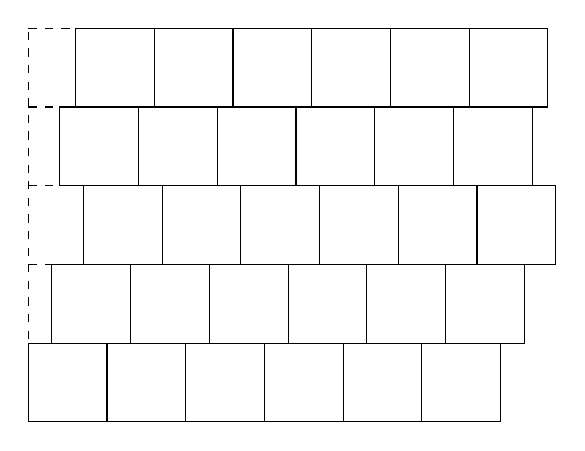
\begin{tikzpicture}[scale=1]
            % Define the tile
            \def\tile{
            % Draw the unit square
            \draw[fill=white] (0,0) rectangle (1,1);
            }

            % Shift list
            \def\BetaMinOne{0}
            \def\BetaZero{0.3}
            \def\BetaOne{0.7}
            \def\BetaTwo{0.4}
            \def\BetaThree{0.6}
            
            

% Axis lines
%\draw[->] (-1.5,0) -- (4.5,0) node[right] {$X$};
%\draw[->] (0,-1.5) -- (0,3.5) node[above] {$Y$};
\draw[dashed] (0,0) -- (6,0);
\draw[dashed] (0,0) -- (0,5);

% Dashed lines at each integer in the x direction
\foreach \x in {0,...,6}
    \draw[dashed] (\x,0) -- (\x,5);

% Dashed lines at each integer in the y direction
\foreach \y in {0,...,5}
    \draw[dashed] (0,\y) -- (6,\y);


            % Draw the tiling pattern
            \foreach \x in {0,1,2,3,4,5}{
            \foreach \y in {0,1,2,3,4}{
                \ifnum\y=0
                    \pgfmathsetmacro{\shiftX}{\x + \BetaMinOne}
                    \pgfmathsetmacro{\shiftY}{\y}
                \fi
                \ifnum\y=1
                    \pgfmathsetmacro{\shiftX}{\x + \BetaZero}
                    \pgfmathsetmacro{\shiftY}{\y}
                \fi
                \ifnum\y=2
                    \pgfmathsetmacro{\shiftX}{\x + \BetaOne} 
                    \pgfmathsetmacro{\shiftY}{\y} 
                \fi
                \ifnum\y=3
                    \pgfmathsetmacro{\shiftX}{\x + \BetaTwo}
                    \pgfmathsetmacro{\shiftY}{\y}
                \fi
                \ifnum\y=4
                    \pgfmathsetmacro{\shiftX}{\x + \BetaThree}
                    \pgfmathsetmacro{\shiftY}{\y}
                \fi
                \begin{scope}[shift={(\shiftX,\shiftY)}]
                \tile % Draw the tile
                \end{scope}
            }}
        \end{tikzpicture}
        %* —————————————————
        \caption{Multiple shifts horizontal}
        \label{fig:multiple_shift_horizontal_tiling}
    \end{subfigure}
    \caption{Text}
    \label{fig:tiling_figures}
\end{figure}


%\section{Proof of Keller's theorem}


%* Ikke si så veldig mye, 
%* Når vi kommer opp i d=2, så har vi åpenbart mer fleksibilitet, selv om Kellers theorem fortsatt er sant. Sånn at vi har jo den begrensningen om at vi må møtes i et heltall. 
%* Vise flexen og referere til kellers - Nei — Ikke begrunne det med Keller, 
%* I to dimensjoner har vi åpenbart større fleksibilitet fordi vi ikke trenger å ha Lattice tiling. Det kan vi vise ved eksempel. Dette ser vi i figur sånn og sånn, men det som også kommer frem så oppfyller jo Alle Kellers theorem, og det vil de også måtte gjøre. Det ville jeg kommentert, uten å, liksom, begrunne det til noe som helst.
%* Dette for å si noe om det (fleksibiliteten vi skal fange) allerede her
%* Vi skal se senere, (kap 5), det vi har tegnet her, strenkt tatt fanger all den fleksibiliteten vi har. Du har ikke noe mer fleksibilitet enn det du har skissert her. Du kan skyve på kolonnene, og du kan skyve på radene. Men det kommer vi tilbake til den og den seksjonen. Prøvd å skiserre. Da viser den figuren her egentlig all den fleksibiliteten vi har, men ikke sagt at du skal skal forklare noe mer om det nå. 


%* Prove the equivalence in chapter five. Here only show. 
%* Chapter 5, the part I showed in the spectra, also classifies all tiling sets.


\end{document}


